%%%%%%%%%%%%%%%%%%%%%%% file template.tex %%%%%%%%%%%%%%%%%%%%%%%%%
%
% This is a general template file for the LaTeX package SVJour3
% for Springer journals.          Springer Heidelberg 2010/09/16
%
% Copy it to a new file with a new name and use it as the basis
% for your article. Delete % signs as needed.
%
% This template includes a few options for different layouts and
% content for various journals. Please consult a previous issue of
% your journal as needed.
%
%%%%%%%%%%%%%%%%%%%%%%%%%%%%%%%%%%%%%%%%%%%%%%%%%%%%%%%%%%%%%%%%%%%
%
% First comes an example EPS file -- just ignore it and
% proceed on the \documentclass line
% your LaTeX will extract the file if required
\begin{filecontents*}{example.eps}
%!PS-Adobe-3.0 EPSF-3.0
%%BoundingBox: 19 19 221 221
%%CreationDate: Mon Sep 29 1997
%%Creator: programmed by hand (JK)
%%EndComments
gsave
newpath
  20 20 moveto
  20 220 lineto
  220 220 lineto
  220 20 lineto
closepath
2 setlinewidth
gsave
  .4 setgray fill
grestore
stroke
grestore
\end{filecontents*}
%
\RequirePackage{fix-cm}

\documentclass[smallextended]{svjour3}

\smartqed  % flush right qed marks, e.g. at end of proof
%
\usepackage{graphicx}

\usepackage[authoryear]{natbib}  %% The order is important

\usepackage[resetlabels]{multibib}
\newcites{inappendix}{Supplementary References}

% \usepackage{alifeconf}

\usepackage{hyperref}

\usepackage{subcaption}

\usepackage{hhline}

\usepackage{amsmath}

\usepackage{rotating}

\usepackage{bibspacing}
\setlength{\bibsep}{0pt plus 0.3ex}

\usepackage{geometry}

\ifdefined\mydraft
\mydraft
\fi

% \usepackage[
%   %subtle
%   moderate
% ]{savetrees}

\graphicspath{{img/}}

% *****************
%  Requirements:
% *****************
%
% - All pages sized consistently at 8.5 x 11 inches (US letter size).
% - PDF length <= 8 pages for full papers, <=2 pages for extended
%    abstracts.
% - Abstract length <= 250 words.
% - No visible crop marks.
% - Images at no greater than 300 dpi, scaled at 100%.
% - Embedded open type fonts only.
% - All layers flattened.
% - No attachments.
% - All desired links active in the files.

% Note that the PDF file must not exceed 5 MB if it is to be indexed
% by Google Scholar. Additional information about Google Scholar
% can be found here:
% http://www.google.com/intl/en/scholar/inclusion.html.


% If your system does not generate letter format documents by default,
% you can use the following workflow:
% latex example
% bibtex example
% latex example ; latex example
% dvips -o example.ps -t letterSize example.dvi
% ps2pdf example.ps example.pdf


% For pdflatex users:
% The alifeconf style file loads the "graphicx" package, and
% this may lead some users of pdflatex to experience problems.
% These can be fixed by editing the alifeconf.sty file to specify:
% \usepackage[pdftex]{graphicx}
%   instead of
% \usepackage{graphicx}.
% The PDF output generated by pdflatex should match the required
% specifications and obviously the dvips and ps2pdf steps become
% unnecessary.


% Note:  Some laser printers have a serious problem printing TeX
% output. The use of ps type I fonts should avoid this problem.


\title{Matchmaker, Matchmaker, Make Me a Match: Geometric, Variational, and Evolutionary Implications of Criteria for Tag Affinity}
\titlerunning{Matchmaker, Matchmaker, Make Me a Match}
\author{
    Matthew Andres Moreno
	  \and Alexander Lalejini
    \and Charles Ofria \\
}

\authorrunning{Moreno et al.} % if too long for running head

\institute{%
  M. A. Moreno \at
  BEACON Center for the Study of Evolution in Action \\
  Department of Computer Science and Engineering \\
  Program in Ecology, Evolutionary Biology, and Behavior \\
  Michigan State University, East Lansing, MI \\
  \email{mmore500@msu.edu}
\and
  A. Lalejini \at
  University of Michigan, Ann Arbor, MI \\
\and
  C. Ofria \at
  BEACON Center for the Study of Evolution in Action \\
  Department of Computer Science and Engineering \\
  Program in Ecology, Evolutionary Biology, and Behavior \\
  Michigan State University, East Lansing, MI \\
}

\date{Received: date / Accepted: date}


\institute{F. Author \at
              first address \\
              Tel.: +123-45-678910\\
              Fax: +123-45-678910\\
              \email{fauthor@example.com}           %  \\
%             \emph{Present address:} of F. Author  %  if needed
           \and
           S. Author \at
              second address
}

\date{Received: date / Accepted: date}

% For several authors from the same institution use the same number to
% refer to one address.
%
% If the names do not fit well on one line use
%         Author 1, Author 2 ... \\ {\Large\bf Author n} ...\\ ...
%
% If the title and author information do not fit in the area
% allocated, place \setlength\titlebox{<new height>} after the
% \documentclass line where <new height> is 2.25in



\begin{document}
\maketitle

\begin{abstract}

Genetic programming and artificial life systems commonly employ tag-matching schemes to determine interactions between model components.
%Criteria to determine affinity between tags %TODO
However, the implications of criteria used to determine affinity between tags with respect to constraints on emergent connectivity, canalization of changes to connectivity under mutation, and evolutionary dynamics have not been considered.
We highlight differences between tag-matching criteria with respect to geometric constraint and variation generated under mutation. 
We find that tag-matching criteria can influence the rate of adaptive evolution and the quality of evolved solutions.
Better understanding of the geometric, variational, and evolutionary properties of tag-matching criteria will facilitate more effective incorporation of tag matching into genetic programming and artificial life systems.
By showing that tag-matching criteria influence connectivity patterns and evolutionary dynamics, our findings also raise fundamental questions about the properties of tag-matching systems in nature.

\keywords{Genetic Programming \and Event-driven Genetic Programming \and Tag-based Referencing \and Module-based Genetic Programming \and Artificial Gene Regulatory Networks}
% \PACS{PACS code1 \and PACS code2 \and more}
% \subclass{MSC code1 \and MSC code2 \and more}

\end{abstract}


\section{Introduction}

TODO \citep{taylor2016open}


\section{Tags and Tag-Matching Metrics}

In all experiments, we used ordered, fixed-length, 32-bit bitstrings as tags.
In experiments where mutations are applied to tags, individual bits are toggled stochastically with uniform per-bit probability.

We call an algorithm used to calculate the match quality between two tags a tag-matching metric.
A tag-matching metric takes two tags as operands and calculates a match distance between them.
We compared five tag-matching metrics, described below.
Full mathematical definitions and implementation details appear in Supplementary Material \citep{Moreno_Ofria_2020}.

\begin{itemize}
  \itemsep0em
  \item \textbf{Hamming Metric}: calculates match distance according to the number of mismatching bits between tags \citep{lalejini2019else, hamming1950error}; Supplementary Section \ref{sec:hammingmetric}.
  \item \textbf{Hash Metric}: calculates a deterministic, but arbitrary, match distance between using the SHA1 cryptographic hash algorithm \citep{eastlake2001us}; Supplementary Section \ref{sec:hashmetric}.
  \item \textbf{Integer Metric}: match distance accumulates scanning upward from the unsigned integer representation of the first tag until the unsigned integer representation of the second tag is reached, wrapping around to zero if necessary \citep{spector2011tag}; Supplementary Section \ref{sec:integermetric}.
  \item \textbf{Bidirectional Integer Metric}: the lesser of integer metric distance calculated scanning upwards (still wrapping around to zero) and integer metric distance calculated scanning downwards (wrapping around at zero); Supplementary Section \ref{sec:integerbimetric}.
  \item \textbf{Streak Metric}: match distance is calcualted as the ratio between the longest contiguously mismatching substring of two bitsets and the longest contiguously matching substring of those bitsets \citep{downing2015intelligence}; Supplementary Section \ref{sec:streakmetric}.\footnote{Our implementation of this metric differs slightly from its original form due to a mathematical error in \citep{downing2015intelligence}.}
\end{itemize}

The hamming and bidirectional integer metrics are included because of their ubiquity in artificial life systems.
The integer metric is included due to its use in seminal work exploring tag-matching in genetic programs \citep{spector2011tag, spector2011s,spector2012tag}
The streak metric was proposed to model large-effect mutations in biology but, to our knowledge, has not yet been formally studied in an evolving system.
The hash metric is introduced in this work in order to investigate the implications of a completely geometrically-unstructured tag-matching scheme.

For consistency of implementation and interpretation, we bound all metrics' tag-matching distances run between 0 (a perfect match) and 1 (a worst match).
We then normalized metrics' match distances so that match distances generated by pairs of randomly generated tags would follow a uniform distribution between 0 and 1.
This allows for an intuitive, consistent interpretation of match distances across all tag-matching metrics.
For example, two tags with a 0.01 match distance are better-matched than 99\% of randomly-generated tag pairs.
Additionally, in situations where raw match distance plays a mechanistic role (for example, probabilistic matching or threshold-based cutoffs), this transformation ensures consistency across metrics.

To accomplish this normalization to a uniform distribution, we sampled 10,000 randomly generated bitstring tag pairs to approximate metrics' raw distribution of match distances.
Then, for all further match distance calculations made using each metric, we calculated corrected distance for a raw distance $r$ as its percentile ranking among the initially-sampled match distances divided by one hundred.
If the exact raw distance $r$ wasn't present in the set of initially sampled match distance, we linearly interpolated between the next-greater and next-lower match distances' percentile rankings.
Supplementary Figure \ref{fig:uniformification} depicts the distributions of match distances between randomly sampled bitstring pairs for each metric before and after this normalization process.




\section{Geometric Analyses} \label{sec:geometric}

In this section, we consider the geometry that tag matching metrics construct over bitstring tag space.


Geometric constraints of tag matching metrics may affect the patterns of tag connectivity that tend to, or even can, arise under a
In a constrained, it is possible for there to be two queries such that no operand can match both queries well.
Likewise, it is possible for there to be two queries such that an operand must match both queries well.

Structure might prove useful to facilitate modularity, where subsets of tag space tend to have associated functionality.
However, it may also constrain the ease (or possibility) at which adaptive variation can be generated.

To get at these questions, we compare distributions of two statistics measuring constraint across our five tag-matching metrics.
\begin{figure}
\begin{center}

\begin{minipage}{0.45\linewidth}
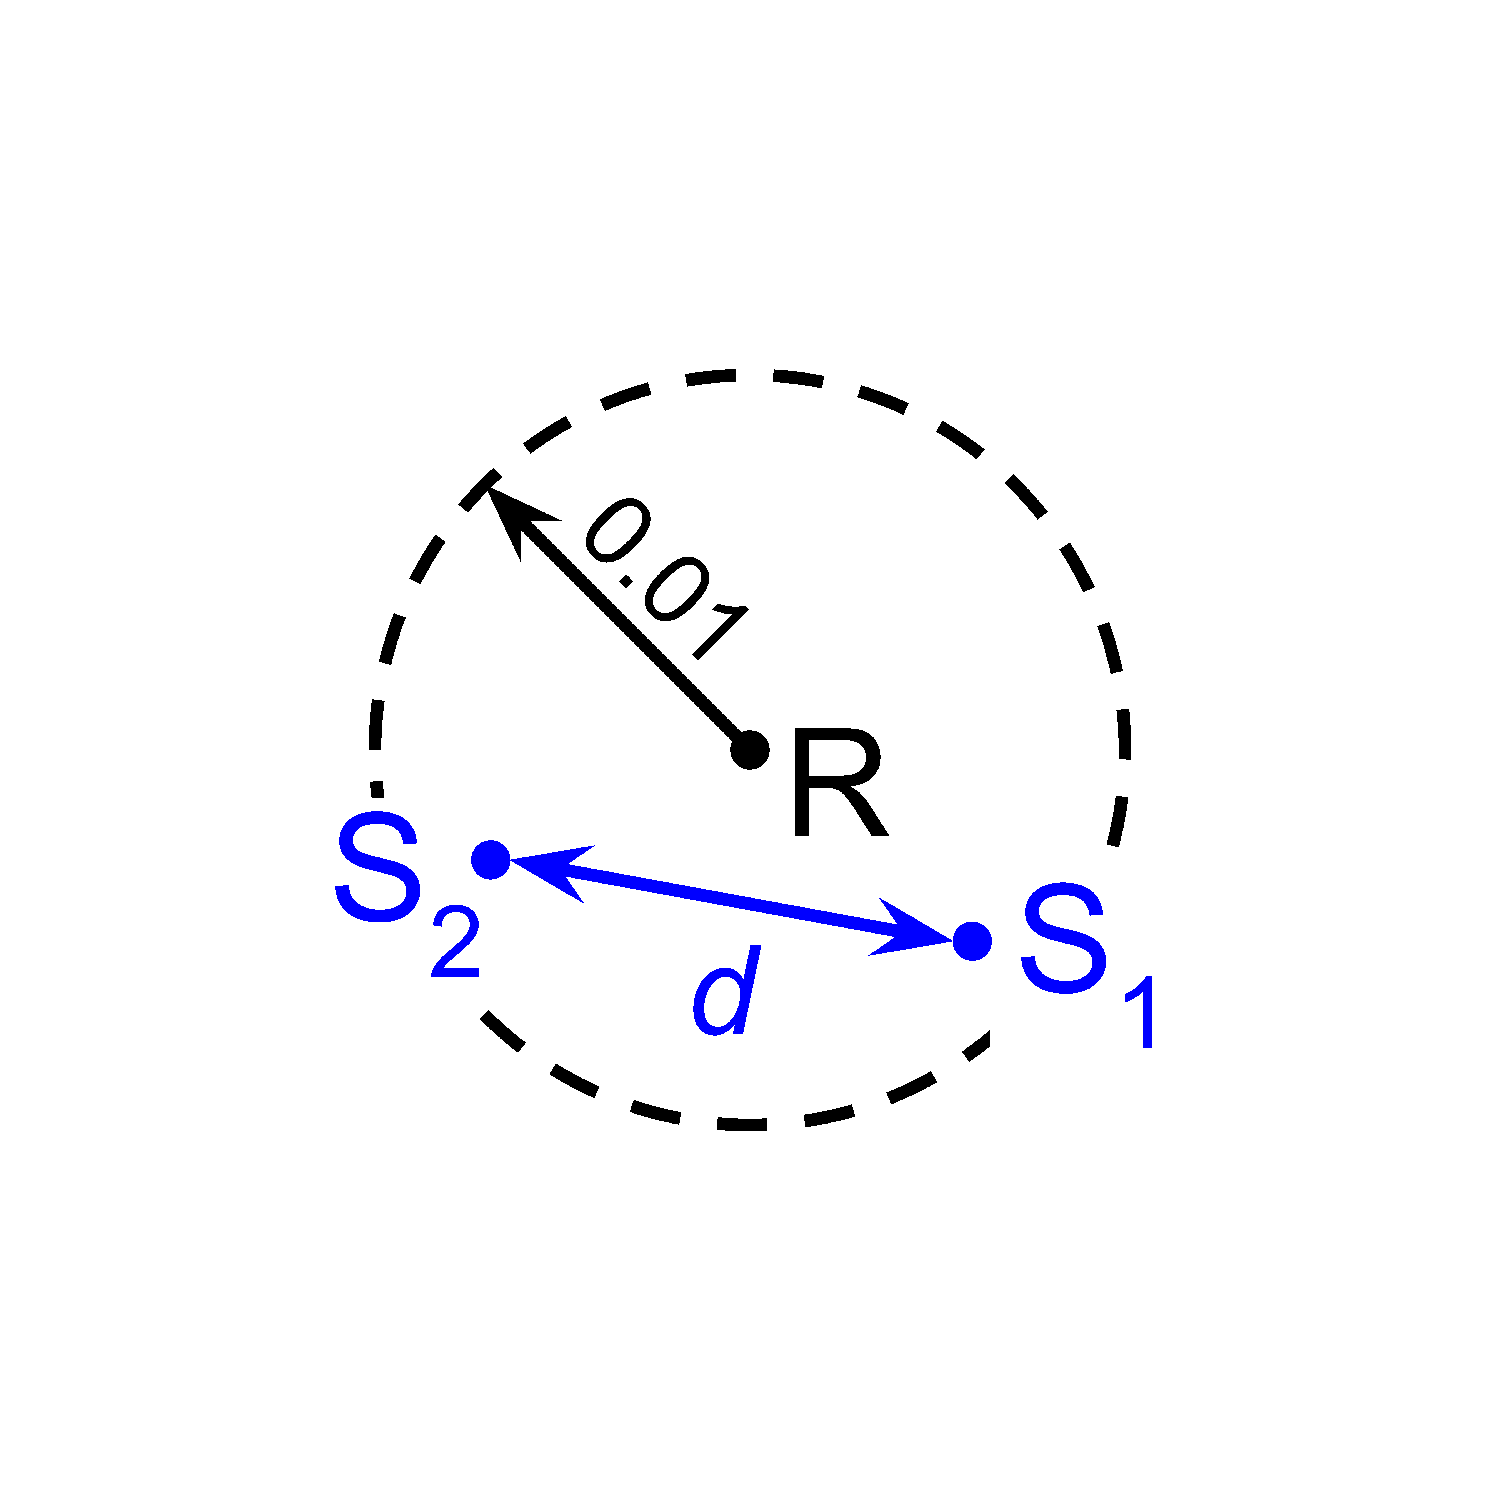
\includegraphics[width=\linewidth]{dimensionality-statistic}
\end{minipage}
\begin{minipage}{0.45\linewidth}
\caption{
The sampling process used to calculate similarity constraint for each metric.
}
\label{fig:dimensionality_measure}
\end{minipage}
\end{center}
\end{figure}


The first statistic we calculate is similarity constraint.
This statistic quantifies the question, "If two tags both match closely to a third tag, will they necessarily match closely with each other?"
To compute this statistic, we randomly sampled 5000 target tags.
Then, for each target tag we randomly sampled tags until we found two secondarily-sampled tags that were within a 0.01 match distance radius to the target.
Finally, we computed the match distance between the pair of seconarily-sampled tags.
Figure \ref{fig:dimensionality_measure}(a) summarizes this process.

The second statistic we calculate is dissimilarity constraint.
This statistic quantifies the question, "If a tag matches a second tag closely and a third tag poorly, will the second and third tag tend to match poorly?"
To compute this statistic, we randomly sampled 5000 target tags.
Then, for each target tag we randomly sampled tags until we found a secondarily-sampled tag that was within a 0.01 match distance radius of the target and a secondarily-sampled tag that was outside a 0.99 match distance radius of the target.
Finally, we computed the match distance between the pair of secondarily-sampled tags.
Figure \ref{fig:dimensionality_measure}(a) summarizes this process.

\subsection{Similarity Constraint}

\begin{figure*}
\begin{center}

\begin{minipage}{0.15\linewidth}
\begin{subfigure}[b]{\linewidth}
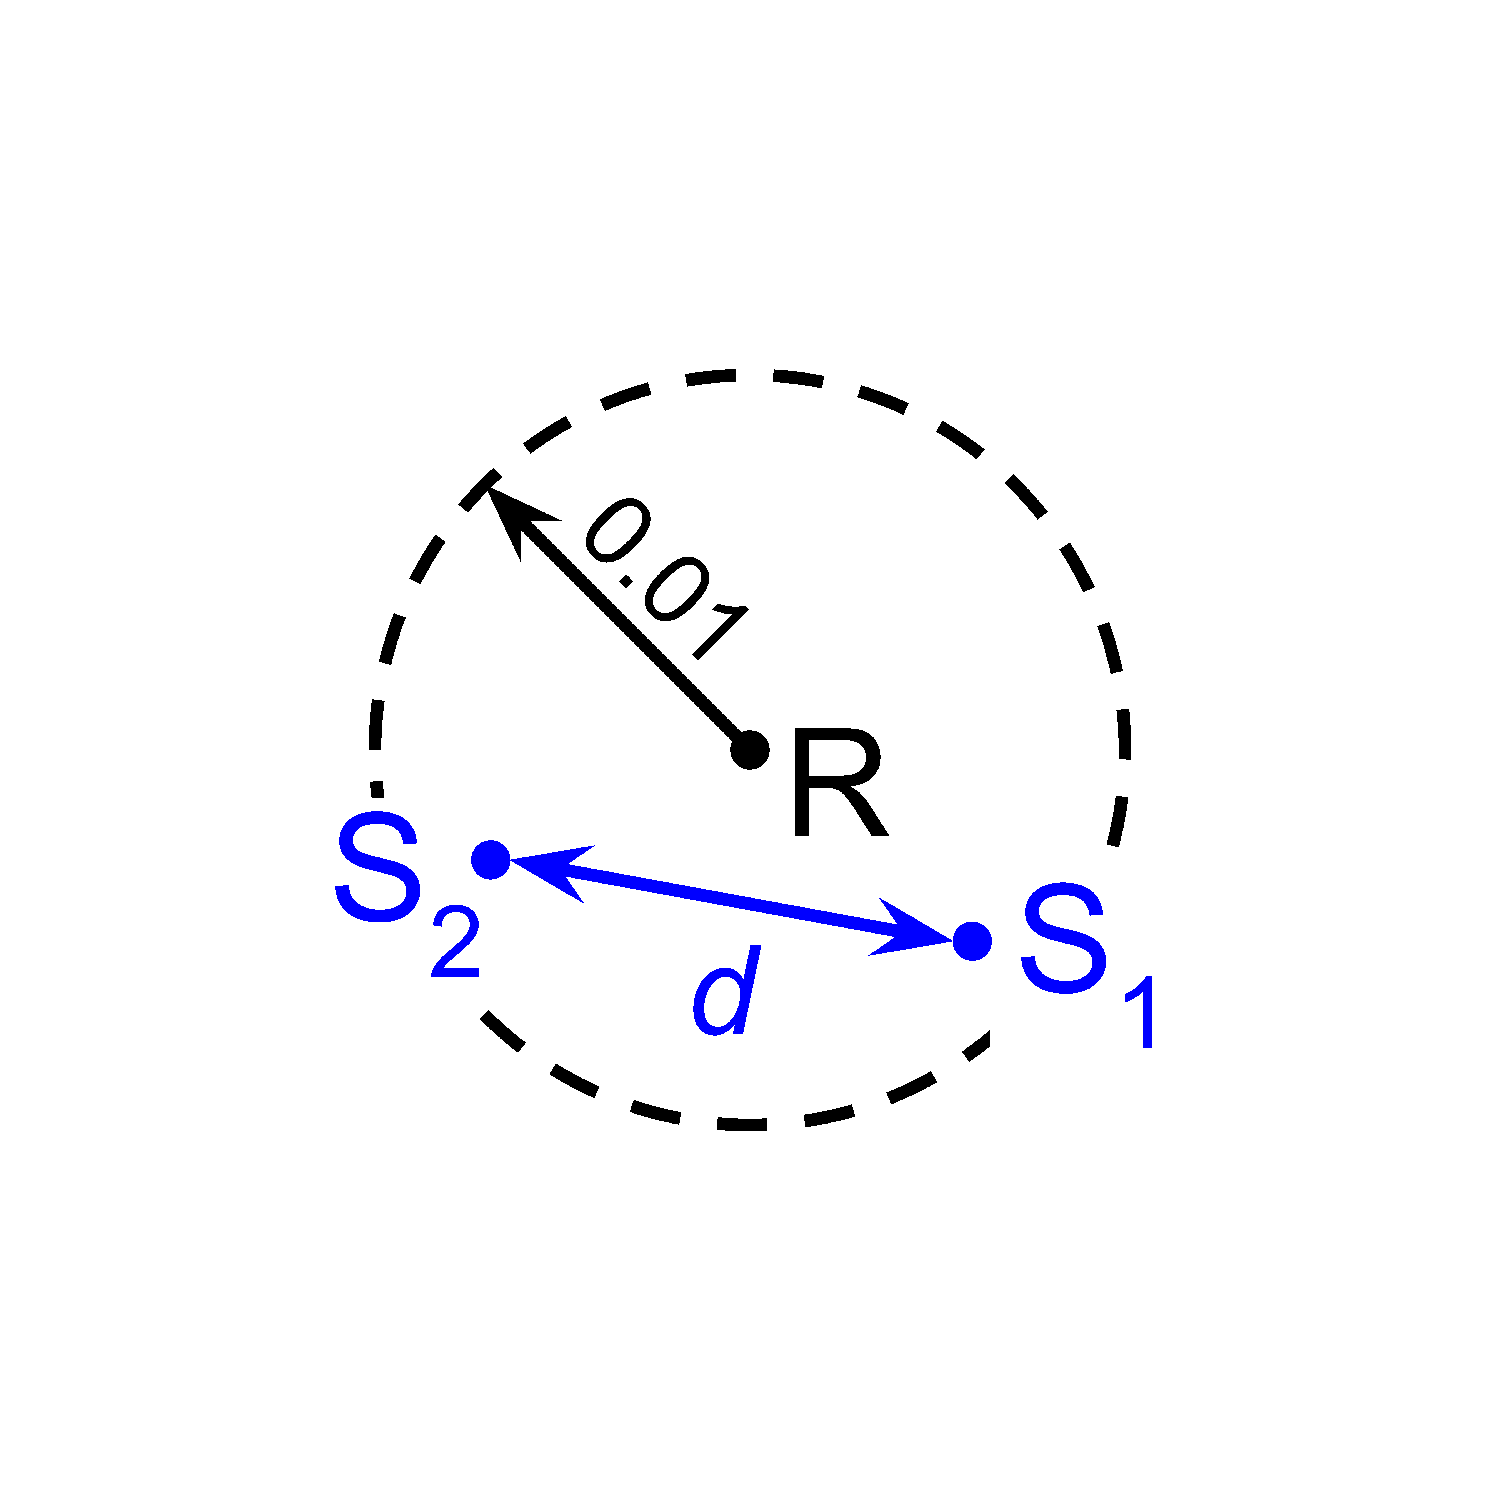
\includegraphics[width=\linewidth]{dimensionality-statistic}
\caption{
The sampling process used to calculate similarity constraint for each metric.
}
\end{subfigure}
\end{minipage}%
\begin{minipage}{0.35\textwidth}
\begin{subfigure}[b]{\linewidth}
\centering
\includegraphics[width=\linewidth]{sphere/bitweight=0dot5+seed=1+title=dimensionality_barplot+_data_hathash_hash=c0f6c5cf854ff253+_script_fullcat_hash=03ce1e318a24a109+ext=}
\caption{
Mean statistic values for each metric.
Error bars represent 95\% confidence intervals.
}
\label{fig:sphere_distnplot}
\end{subfigure}
\end{minipage}%
\begin{minipage}{0.5\linewidth}
\begin{subfigure}[b]{\linewidth}
\centering
\includegraphics[width=\linewidth]{sphere/bitweight=0dot5+seed=1+title=dimensionality_distnplot+_data_hathash_hash=c0f6c5cf854ff253+_script_fullcat_hash=03ce1e318a24a109+ext=}
\caption{
Statistic distribution, where each horizontal bar sliver represents one independent observation.
}
\label{fig:sphere_barplot}
\end{subfigure}
\end{minipage}

\caption{
Dimensionality statistic measured as distances between two tags sampled from within 0.01 match distance of a third tag.
}
\label{fig:sphere}

\end{center}
\end{figure*}


In a euclidean space, the similarity constraint metric would correspond to the average distance between points uniformly sampled from inside a ball (e.g., in two dimensions a circle, in three dimensions a sphere, etc.).
Average distance between such points increases with dimensionality.
For reference, in a one dimensional Euclidean space similarity constraint would measure approximately 0.0067.
In a two dimensional Euclidean space, it would measure approximately  0.0091.
In 32 dimensions, it would measure 0.0137 \citep{dunbar1997average}.

Figure \ref{fig:sphere_barplot} provides our estimate of the similarity constraint statistic for each metric, with error bars representing a 95\% confidence interval.
Figure \ref{fig:sphere_distnplot} shows the distribution of the similarity constraint statistic values among the 5000 replicate samples in greater detail.

For the bidirectional integer metric, we measured the similarity constraint statistic as 0.0068.
This falls in line with expectation: this metric is essentially identical to a one-dimensional Euclidean space.
As shown in Figure \ref{fig:sphere_distnplot}, the secondarily-sampled match distances are all bounded by the diameter of 0.02.
This metric not only exhibits tight similarity constraint in the mean case, but also permits no outliers to the similarity constraint.

The unidirectional integer metric exhibits much looser similarity constraint in the mean case.
We estimated this value as 0.5092.
However, this looser similarity constraint appears to be an artifiact of averaging between two very tight constraints: a tight constraint to 0 in one case and a tight constraint to 1 in the other.
In Figure \ref{fig:sphere_distnplot}, you can clearly see that all sampled cases fall under one of these umbrellas.
This phenomenon results from the asymmetrical definition of the metric.
If you sample pairs of similar values, half will be in ascending order (resulting in a match distance close to 0) and half will be in descending order, (resulting in a wraparound search and a match distance close to 1).
Averaging these outcomes out yields the observed mean value of 0.5.
The integer metric appears to allow for closely related tags to either very strongly match or very weakly match, but permits no intermediate outcomes.

The hamming metric exhibits a broader range of sampled similarity constraint values than the integer metrics.
We estimated mean similarity constraint as 0.1627, looser than the bidirectional integer metric.
As shown in Figure \ref{fig:sphere_distnplot}, many secondarily-sampled tag pairs are biased towards low match distances.
However, secondarily-sampled tag pairs that break this low match distance constraint are also not uncommon.
Among our 5,000 trials, we observed distances between secondarily-sampled tags as high as 0.7499.

Why is our estimate of the hamming metric similarity constraint statistic so much higher than expected in a 32-dimensional Euclidean space?
This phenomenon appears to be due to the normalization process we applied to map raw match distances to a uniform distribution.
We also calculated this statistic for the raw hamming metric without normalization.
For practical reasons, we increased the radius of our sampling sphere to 0.25.
(Only the exact target 32-bit tag satisfies within-sphere constraint with a sampling radius of 0.01.)
In 32-dimensional euclidean space with a sampling radius of 0.25, the expected distance between sampled points is 0.3415.
Our estimate of the raw hamming metric's similarity constraint statistic falls nearly in line with expectation at 0.3312.

The streak metric exhibited the next-loosest similarity constraint statistic with a mean value sampled at 0.2813.
For this metric, we observed distances between secondarily-sampled tags as high as 0.9993.
The streak metric retains some geometric constraint in the mean case, but outliers that strongly break similarity constraint are also not uncommon.

Like the integer metric, the hash metric also exhibits looser similarity constraint in the mean case.
We estimated this value as 0.5083 for the hash metric.
However, unlike the integer metric, intermediate secondarily-sampled match distances are also are possible.
In fact, secondarily-sampled match distances are uniformly distributed.
This is exactly as we would expect:
given any particular set of operands, a well-behaved hash function should yield a uniform distribution of hash results.
The hash metric exhibits no geometric structure and total geometric flexibility.

\subsection{Dissimilarity Constraint}

\begin{figure}[!htbp]

\begin{center}
\begin{subfigure}[b]{\linewidth}
\begin{minipage}{0.5\linewidth}

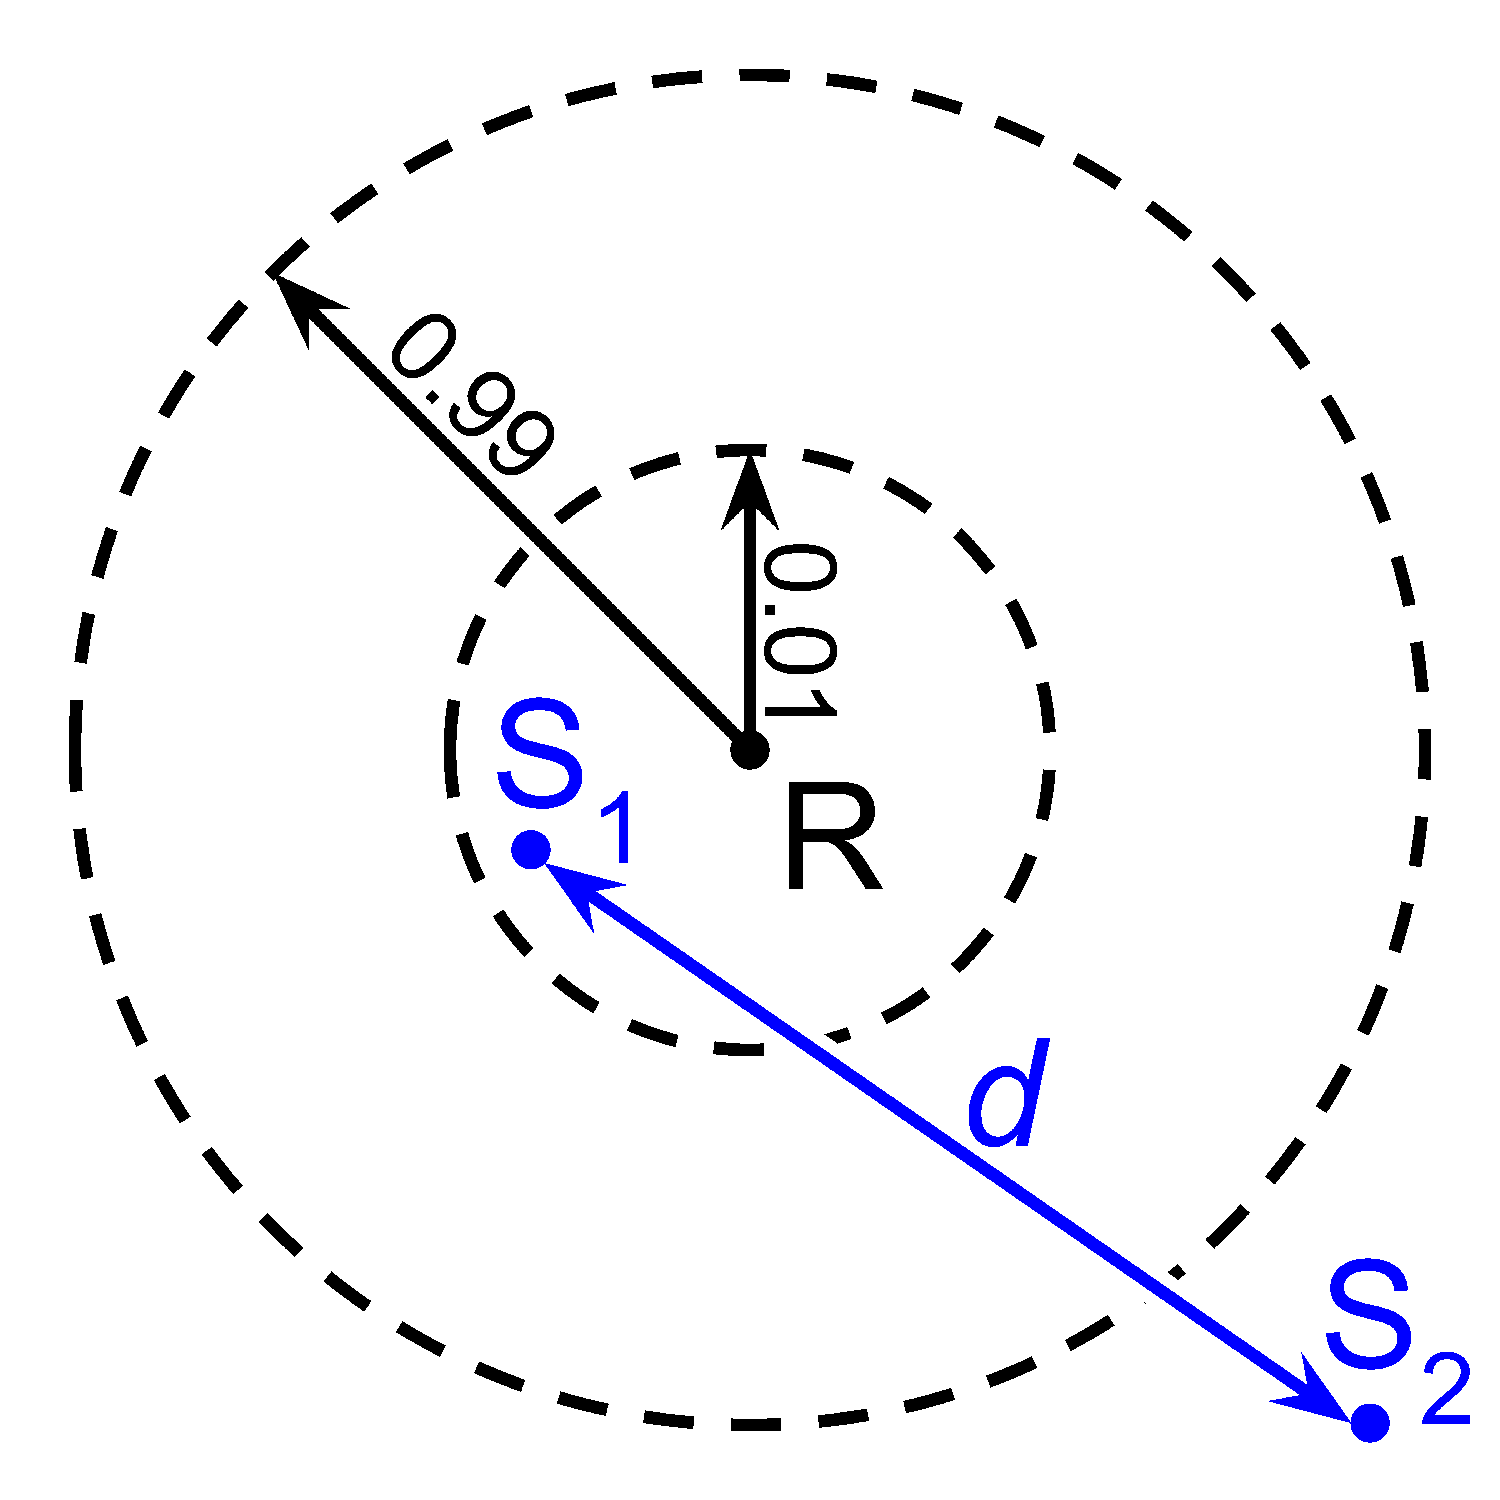
\includegraphics[width=0.75\linewidth]{img/elasticity-statistic}

\end{minipage}
\begin{minipage}{0.5\linewidth}
\caption{
Sampling process used to measure dissimilarity constraint.
First, a target tag $R$ was randomly sampled.
Then, tags were randomly drawn until a tag $S_1$ with distance to $R$ less than 0.01 was obtained.
Next, tags were randomly drawn until a tag $S_1$ with distance to $R$ more than 0.99 was obtained.
Finally, dissimilarity constraint was measured as the distance $d$ between $S_1$ and $S_2$.
}
\label{fig:dissimilarity_statistic}
\end{minipage}

\end{subfigure}

\begin{subfigure}[b]{\linewidth}
\begin{minipage}{0.6\linewidth}
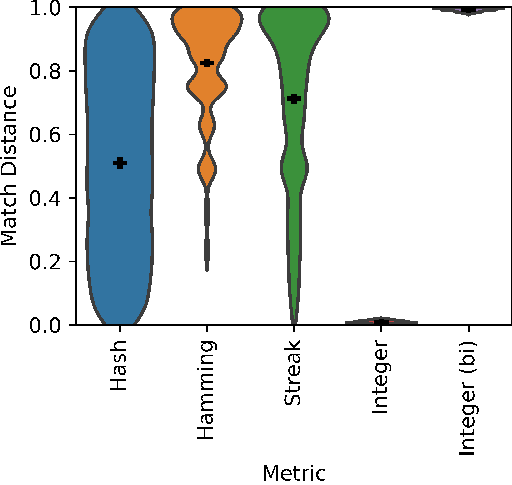
\includegraphics[width=\linewidth]{img/sphere_reverse/bitweight=0dot5+seed=1+title=dimensionality_violinplot+_data_hathash_hash=93f97a11cb443d35+_script_fullcat_hash=d1692569f79e33f8+ext=}
\end{minipage}
\begin{minipage}{0.35\linewidth}
\caption{
Mean dissimilarity constraint values for each metric.
Horizontal ticks represent means.
Error bars represent 95\% confidence intervals.
Violin plots show kernel density estimates for distribution of dissimilarity constrant.
}
\label{fig:sphere_reverse_distnplot}
\end{minipage}
\end{subfigure}
\begin{subfigure}[b]{\columnwidth}
\centering
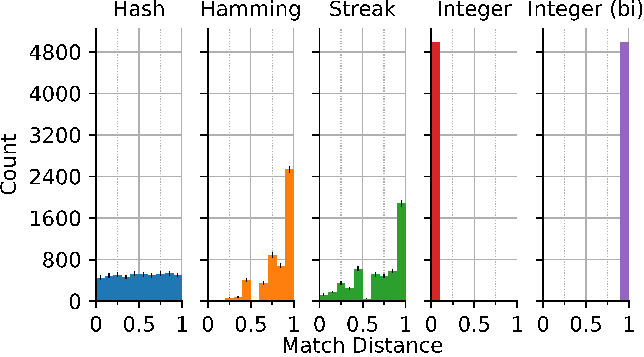
\includegraphics[width=\columnwidth]{img/sphere_reverse/bitweight=0dot5+seed=1+title=dimensionality_distnplot+viz=hist+_data_hathash_hash=93f97a11cb443d35+_script_fullcat_hash=cda229fb13f5a152+ext=}
\caption{
Frequency of sampled dissimilarity constraint values in each match distance decile.
Error bars are 95\% confidence intervals calculated using the Wilson score method with continuity correction \citep{newcombe1998two}.
}
\label{fig:sphere_reverse_barplot}
\end{subfigure}

\caption{
Dissimilarity constraint of tag-matching metrics.
Figure \ref{fig:dissimilarity_statistic} summarizes the sampling process used to measure similarity constraint.
Figures \ref{fig:sphere_reverse_barplot} and \ref{fig:sphere_reverse_distnplot} compare distributions of similarity constraint across metrics.
Supplementary Figure \ref{fig:sphere_reverse_supp} visualizes the cumulative distribution of all sampled dissimilarity constraint values for each metric.
}
\label{fig:sphere_reverse}

\end{center}
\end{figure}


Figure \ref{fig:sphere_barplot} provides our estimate of the dissimilarity constraint statistic for each metric, with error bars representing a 95\% confidence interval.
Figure \ref{fig:sphere_distnplot} shows the distribution of the dissimilarity constraint statistic values among the 5000 replicate samples in greater detail.

These results tell a story across metrics very to the simiarity constraint results.
The hash metric exhibited no geometric structure.
The streak metric exhibited some geometric structure in the mean case (mean secondarily-sampled distance 0.7127), but outcomes that strongly broke geometric constraints were also observed (we observed distances between secondarily-sampled tags as low as 0.0002).
The hamming metric exhibited stronger geometric structure in the mean case (mean secondarily-sampled distance 0.8248) and had less extreme tail-end outcomes (we observed match distances between the secondarily-sampled tags only as low as 0.2355).
The bidirectional integer metric was highly constrained in both the mean and tail-end cases.
The smallest distance between secondarily-sampled tags was 0.9802.
Again, the unidirectional integer metric exhibited a quirky result due to its noncommutative nature.
The mean distance between secondarily-sampled tags was 0.0100.
As shown in Figure \ref{fig:sphere_distnplot}, all secondarily-sampled distances oberved with this metric were extremely small.
Under this metric, if you sample a tag that is close to a target it will be numerically slightly larger than the target.
Likewise, if you sample a tag that is very far from a target, it will be numerically slightly smaller than the target (due to wraparound).
Then, explaining this counterintuitive result, the distance from the slightly smaller to the larger tag will be small.



\section{Variational Analysis} \label{sec:variational}

For each tag-matching metric, we performed single-step mutational analyses to examine the local mutational neighborhood of loosely-affiliated and tightly-affiliated tag pairs and a mutational walk analysis to survey the broader mutational landscape.

\subsection{Single-Step Mutations}

\begin{figure}
\begin{center}

\includegraphics[width=\columnwidth]{img/mutational_step/bitweight=0dot5+seed=1+title=low-mutational-step+_data_hathash_hash=95a57768de56995a+_script_fullcat_hash=78f9965681c3a44b+ext=}
\caption{
Distributions of mutation effects on match distance for loosely matched (pre-mutation match distance $> 0.5$) and tightly matched (pre-mutation match distance $< 0.01$) tag pairs.
Each distribution visualization arranges individually sampled observations of mutation outcome from an independently sampled tag pair (thin horizontal bars) vertically in descending order.
The $y$ axis can be interpreted as ranging form the 0th percentile of outcomes (bottom) to 100th percentile (top) with horizontal bar width showing the mutation effect size at a certain percentile.
Mutations that increase affinity are colored blue and mutations that decrease affinity are colored red.
Solid lines indicate the median between mutations that increase match distance and mutations that decrease match distance.
Dashed lines demarcate the boundaries between non-neutral and perfectly-neutral mutations.
}
\label{fig:mutational_step}

\end{center}
\end{figure}


Figure \ref{fig:mutational_step} visualizes the distribution of changes to match distance from single-bit mutations.

The distribution of mutational perturbations on loosely-affiliated tag pairs reflects the effects of one-step mutations on tags without pre-existing affinity.
To measure the distribution of mutational perturbations on loosely-affiliated tag pairs We began by sampling a target tag and then randomly sampled candidate tags until we found a second tag with a match distance $> 0.5$.
We recorded the match distance between our tag pair, applied a one-bit mutation to the secondary tag, and then measured the match distance between the tag pair again.
We repeated this process to generate 5000 samples.
Mutational perturbation was calculated as the difference between the match distances.
A negative mutational perturbation indicates a decrease in match distance and, therefore, an increase in match quality.

We measured the distribution of mutational perturbations on tightly-matched tag pairs similarly, except we uniformly sampled secondary candidate tags until we found a second tag with match distance $< 0.01$.
This distribution reflects the effects of one-step mutations on tags with pre-existing affinity.

For both tightly- and loosely-affiliated tag pairs under the integer and bidirectional integer metrics, most mutations caused very small changes in match distance.
These mutations toggle least-significant bits of the tag's integer representation.
However, under these metrics, a small fraction of mutations affecting more-significant bits of the integer representation have a much stronger effect.
Single-step mutations occasionally occur that strongly couple loosely-affiliated tag pairs or strongly decouple tightly-affiliated tag pairs.
In particular, the unidirectional integer metric appears to exhibit more frequent strong decoupling mutations than the bidirectional integer metric, presumably due to its non-commutative quirks.

The streak metric exhibits a large fraction of perfectly neutral outcomes under mutation.
These perfectly-neutral mutations presumably affect regions of the bitstring neither involved in the longest-matching streak nor in the longest-mismatching streak.
The streak metric exhibits a fatter tail of mutational magnitude for mutations that couple loosely-affiliated tags than the integer metrics. %TODO - consider word change for 'fatter'
In addition, the most extreme mutational outcomes that couple loosely-affiliated tags appear to be of a comparable magnitude to those under the integer metrics.
Mechanistically, this might be due to mutations that disrupt longest-mismatching streaks.
However, one-step mutations that decouple tightly-affiliated tags do not appear as potent.
This might be because achieving a very poor match requires both increasing longest-mismatching streak length and decreasing longest-matching streak length.

The hamming metric exhibits a generally uniform magnitude of match-distance changes under mutation.
High-magnitude one-step mutations do not occur under this metric.
(Without normalizing match distance to a uniform distribution for randomly-sampled tags, all hamming metric mutations would be of exactly the same magnitude, either increasing or decreasing the count of matching bits by 1.)

The hash metric exhibits the fattest tails of mutational magnitude of all metrics.
Extreme-effect one-step mutations are plentiful under this metric.
Interestingly, compared to other metrics, the hash metric exhibits a greater fraction of mutations that decouple tightly-affiliated tags and a greater fraction of mutations that couple loosely-affiliated tags.
This might be due to the hash metric's lack of geometric structure.
Because all one-step mutations uniformly sample a new match distance, 99\% of one-step mutations on tightly-affiliated tags will result in a looser coupling.
Similarly, approximately 75\% of one-step mutations on loosely-affiliated tags will result in a tighter coupling.

\subsection{Mutational Walks}

\begin{figure}
\begin{center}

\includegraphics[width=\columnwidth]{{{mutational_walk/bitweight=0.5+seed=1+title=mutational_walk_barplot+_data_hathash_hash=ff15c8831d4f9288+_script_fullcat_hash=c872df869f05035a+ext=}}}
\caption{
TODO
}
\label{fig:mutational_walk_barplot}

\end{center}
\end{figure}


Figure \ref{fig:mutational_walk_barplot} shows how match distance increases of mutational walks from initially exactly-equivalent tags.
%Match distances from each metric along these walks are compared side-by-side for exponentially-spaced mutational steps.
To conduct a mutational walk, we first randomly generated a starting tag.
Then, we sequentially applied 65 randomly-chosen one-step bit flip mutations, with back mutation allowed.
At each step along the walk, we measured match distance to the original starting tag.
We analyzed 1000 replicate mutational walks for each metric.

Under the hash metric, bitwise equivalent tags do not exhibit low match distance.
So, the mutational walk begins with and then maintains a mean match distance of 0.5.
Under the integer metric, half of mutational steps cause a wrap around effect, immediately spiking the average match distance to 0.5.
% Supplementary Figure \ref{fig:mutational_walk_lineplot} shows match distance variance decreasing as the walk proceeds away from match distances biased towards 0 or 1 \cite{Moreno_Ofria_2020}.
The bidirectional integer metric proceeds away from match distance 0 the next quickest, presumably due to large-effect mutations affecting significant bits. %TODO - added 'to' after '0' - confirm that sentence is correct
% - @AML: 'away from match distance 0 to the next quickest' => to what? I think 'to' breaks the sentence, removing.

The streak metric proceeds away from match distance 0 the second-slowest, trailed only by the hamming metric. %TODO - added 'to' after '0' - confirm that sentence is correct
% @AML: see above comment about 'to'
Interestingly, this result contradicts Downing's presentation of the streak metric in \citep{downing2015intelligence}, in which he suggests that the streak metric exhibits greater robustness because its match distance diverges more slowly under a mutational walk.
This discrepancy is presumably due to our normalization to ensure a uniform distribution of raw match scores between 0 and 1.




\section{Evolutionary Analysis}

\begin{figure*}
\begin{minipage}{0.25\textwidth}

\begin{subfigure}[b]{\linewidth}
\centering
\includegraphics[width=\linewidth]{img/gp_results/panel-cst-sols.pdf}%
\caption{
changing-singal task
}
\label{fig:cst-sols}
\end{subfigure}

\begin{subfigure}[b]{\linewidth}
\centering
\includegraphics[width=\textwidth]{img/gp_results/panel-dst-sols.pdf}%
\caption{
directional-signal task
}
\label{fig:dst-sols}
\end{subfigure}
\begin{subfigure}[b]{\linewidth}
\centering
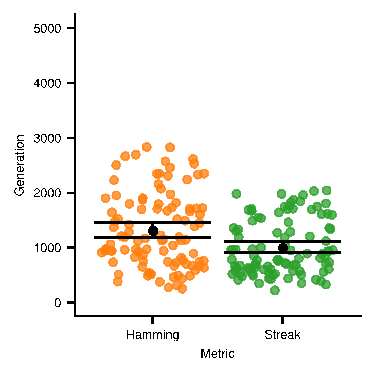
\includegraphics[width=\textwidth]{img/gp_results/panel-dst-times.pdf}%
\caption{
directional-signal task
}
\label{fig:dst-times}
\end{subfigure}

\label{fig:gp_results}

\end{minipage}%
\begin{minipage}{0.75\textwidth}

\begin{subfigure}[b]{\linewidth}
\includegraphics[width=\linewidth]{img/target_evolve/viz=max-fitness-bar+_data_hathash_hash=673d309ab90e91d1+_script_fullcat_hash=6c7848b1ac357236+ext=}
\caption{
graph-matching task
}
\label{fig:evolve_bests}
\end{subfigure}

\caption{
Evolutionary analyses of tag-matching metrics.
All show each metrics' best-performing mutation rate.
Figures \ref{fig:cst-sols} and \ref{fig:dst-sols} show the numbers of replicates that produced a complete task solution to the changing-signal and directional-signal task respectively.
Figure \ref{fig:dst-times} show the number of generations elapsed for the first 100 replicates to produce a complete solution to the directional-signal task.
Error bars indicate bootstrapped 95\% confidence intervals around the mean generation.
Figure \ref{fig:evolve_bests} shows maximum fitness by update over replicate runs on the graph-matching task.
Error bars represent 95\% confidence intervals.
}
\end{minipage}
\label{fig:evocomposite}
\end{figure*}

We performed two evolutionary experiments to characterize our five tag-matching metrics.
The first, in which we evolved sets of tags to form connectivity patterns matching a target graph, allowed us to isolate how tag-matching constraints (how many tag-matching criteria that must be simultaneously fulfilled) affected the rate of adpative evolution and the solution quality of evolved solutions.

The second, in which we evolved full-fledged SignalGP programs that used tag matching to control module activation, allowed us to investigate if tag-matching metrics exhibited different performance characteristics in a more generalized, complex domain.
% @AML: dumping this text here. still needs to be cut down.
We investigate the success of each of the five tag-matching schemes in the context of SignalGP on two diagnostic GP problems: the changing-signal and the directional-signal tasks.
The changing-signal task evaluates how well a GP representation can associate a set of distinct behavioral responses each with a particular environmental cue.
The directional-signal task evaluates how well a representation facilitates signal-response plasticity (\textit{i.e.}, the ability to alter responses to repeated cues during the program's lifetime).

\subsection{Matching a Target Graph}

In this evolutionary experiment, we evolved genomes consisting of 32 bitstring tags to establish a pattern of connectivity mirroring that of a randomly-generated target bipartite graph.
Each bitstring tag in a genome corresponded to a node in the target graph.
Half of the graph nodes, comprising one partition of the graph, were designated as queries.
The other half of the graph nodes, comprising the other partition of the graph, were designated as operands.
To evaluate the fitness of a genome, we harvested the tags corresonding to the operand nodes of the graph and placed them into a tag-matching data structure.
This data structure allowed us to calculate the best matches among the set of operand tags for each query tag (the operand tags with minimal match distance to that query).
For each query tag, we recorded as many match results as outgoing connections from the corresponding node in the target graph.
Fitness was calculated as the fraction of operand tag results that corresponded to nodes in the target graph that queries connected to.

We controlled the amount of tag-matching constraint imposed by the target graph by manipulating:
\begin{enumerate}
  \item the mean number of edges per node (graph degree), and
  \item whether edges were assigned evenly such that all nodes had identical degree (regular structure) or were assigned at random, likely causing some nodes to have high degree (irregular structure).
\end{enumerate}
We tested target graphs mean degree 1 and 2 and both regular and irregular construction.
Regular, degree 1 graphs imposed the least tag-matching constraint.
Degree 2 graphs imposed the most tag-matching constraint.
Supplementary Figure \ref{fig:graph_layouts} provides a visual depiction of these graph layouts.

For each target graph configuration, we surveyed each metric's performance over ten per-bit mutation rates ranging from 0.75 expected mutations per genome to 16.0 expected mutation rates per genome.
For each metric and target graph configuration combination, we chose the most favorable mutation rate defined by sum population-maximum fitness across updates.\footnote{
Supplementary Figure \ref{fig:evolve_mutsweep} summarizes evolutionary performance of metrics across mutation rate/target graph configurations.
All metrics show evidence of a performance maxima within the range of mutation rates surveyed, except for the hash metric on the regular target graph of degree 1 where peak performance was observed on the lowest sampled mutation rate.
}
We ran 100 replicate 512-generation evolutionary runs for each mutation rate/target graph/metric combination.
We used a well-mixed population of size 500 and tournament size 7.

Figure \ref{fig:evolve_bests} plots population-maximum fitness across evolutionary runs.
The fitness trajectory of each metric under its best-performing mutation rate is shown.

Surprisingly, the hash metric enables faster adaptive evolution than all other metrics toward matching the least-constrained target graph, regular structure with mean degree 1 (non-overlapping 95\% CI).
On more-constrained target graphs with mean degree 2, the hash metric's advantage in rapid adaptive evolution disappears.
In fact, on the most-constrained target graph (irregular structure with mean degree 2) the hash metric yields significantly lower-quality solutions at the end of evolutionary runs than the streak and hamming metrics.

The integer and bidirectional integer metrics successfully evolve connectivity patterns matching the unconstrained target graph (regular structure with mean degree 1) but yield lower-quality solutions than other metrics on constrained target graphs (non-overlapping 95\% CI).

The streak metric facilitates slightly faster adaptive evolution than the hamming metric, especially on mean degree 2 target graphs (non-overlapping 95\% CI).

We performed the same evolutionary experiment with 64-node target graphs and observed qualitatively similar results (Supplementary Figure \ref{fig:evolve_bests64}).

% @AML: I don't like this heading. 
\subsection{Evolving tag-based genetic programs}

% -- Introduce SignalGP --
We explore the implications of different tag-matching metrics using SignalGP, a tag-based genetic programming (GP) representation \citep{lalejini2018evolving}.
SignalGP employs tags to enable signal-driven program execution where tags specify the relationship between signals and signal-handlers (program modules).
In SignalGP, programs are segmented into modules (functions) that may be automatically triggered by exogenously- or endogenously-generated signals.
Each module in SignalGP associates a tag with a linear sequence of instructions.
SignalGP makes explicit the concept of signals (events), which comprise a tag and, optionally, signal-specific data.
Signals trigger the module with the closest matching tag (according to a given tag-matching scheme), using any signal-associated data as input to the triggered module.

The SignalGP instruction set, in addition to including traditional GP operations, allows programs to generate internal signals, broadcast external signals, and otherwise work in a tag-based context.
Instructions contain arguments, including an evolvable tag, that may modify the instruction's effect, often specifying memory locations or fixed values.
Instructions may refer to program modules using tag-based referencing; for example, an instruction may trigger the execution of a program module using the instruction's tag to specify which module to trigger.
SignalGP also supports genetic regulation with promoter and repressor instructions that, when executed, allow programs to adjust how well subsequent signals match with a target function (specified with tag-based referencing). % todo - cite regulation paper
% TODO - when reviews come back, cite regulation paper?
See \citep{lalejini2018evolving} for a more detailed description of SignalGP.

% -- Changing-signal task --

\subsubsection{Solving a minimally constrained problem}

The changing-signal task requires programs to express a distinct response to each of $K$ environmental signals (each signal has a unique tag).
Programs express a response by executing one of $K$ response instructions.
Successful programs can `hardcode' each response with the appropriate environmental signal, ensuring that each environmental signal's tag best matches the function containing the correct response.
Thus, SignalGP module tags are minimally constrained --- each needs to only match with a single environmental signal.

During evaluation, we afford programs 64 time steps to express the appropriate response after receiving a signal.
Once a program expresses a response or the allotted time expires, we reset the program's virtual hardware (resetting all executing threads and thread-local memory), and the environment produces the next signal.
Evaluation continues until the program correctly responds to each of the $K$ environmental signals or until the program expresses an incorrect response.
During each evaluation, programs experience environmental signals in a random order; thus, the correct \textit{order} of responses will vary and cannot be hardcoded.

% Experiment overview
% @AML: currently, this section outsources A LOT of the configuration details to the supplement. Need to discuss what level of detail we want to go into here.
We compared the performance of SignalGP with each of the Hamming, Hash, Integer, Bidirectional Integer, and Streak tag-matching metrics.
For each metric, we evolved 200 replicate populations (each with a unique random number seed) of 500 asexually reproducing programs in an eight-signal environment ($K=8$) for 100 generations.
We identified the most performant per-bit tag mutation rates (from a range of possible mutation rates) for each metric on the changing-signal task (these data are available in supplemental material [CITE]): 0.01 for the Hamming and Streak metrics, 0.002 for the Hash metric, and 0.02 for the Integer and Bidirectional Integer metrics.
Aside from tag mutation rate, the overall configuration used for each metric was identical.
We limited tag variation in offspring to tag mutation operators (bit flips) by initializing populations with a common ancestor program in which all tags are identical and by disallowing mutations that would insert instructions with random tags.
Our supplemental material gives the full configuration details for this experiment, including a guide for replication [CITE].

\begin{figure*}
  \begin{center}

  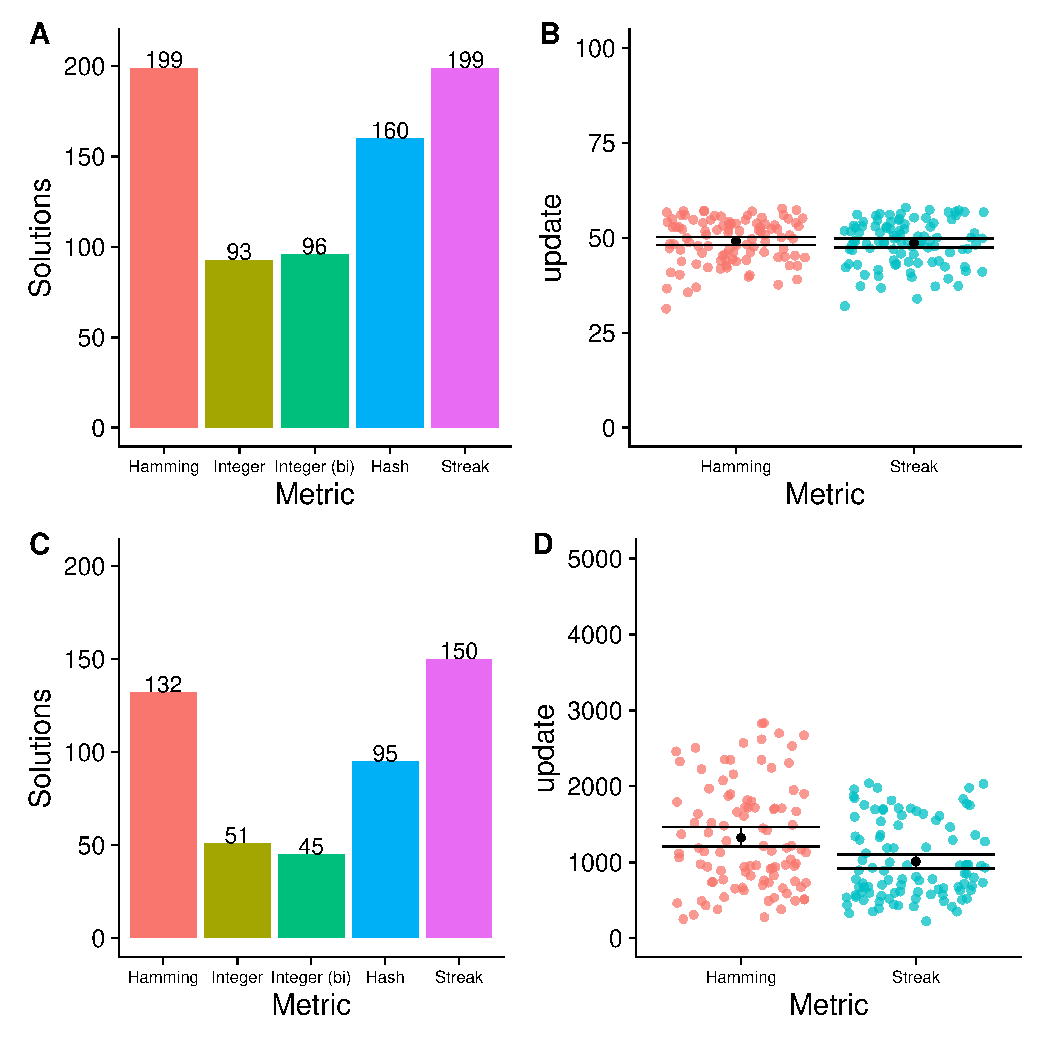
\includegraphics[width=\columnwidth]{img/gp_results/gp_results_panel}
  \caption{
  Todo - caption. A, B are changing-signal task; C, D are directional signal task.
  }
  \label{fig:gp_results}

  \end{center}
  \end{figure*}

Figure \ref{fig:gp_results} gives the number of replicates that produced a successful SignalGP program (\textit{i.e.}, capable of achieving maximum fitness) for each tag-matching metric on both the changing-signal task.
We compared the number of successful replicates across metrics using a pairwise Fisher's exact test (with a Holm correction for multiple comparisons).

The Hamming and Streak metrics performed significantly better than all other metrics ($p < 5\times10^{-11}$); however, there was no significant difference in performance between the Hamming and Streak metrics.
To assess whether the Streak metric produced solutions in fewer generations than the Hamming metric, we ran 200 new replicates of each condition until 100 replicates produced a solution and recorded the number of generations that elapsed (Figure \ref{fig:cst-times}).
We found no difference in generations elapsed between the Hamming and Streak metrics.

We observed no difference in success between the Integer and Bidirectional Integer metrics.
The Hash metric performed better than expected, significantly outperforming both Integer metrics ($p < 4\times10^{-10}$).
Intuitively, the Hash metric maximizes the amount of phenotypic variation (\textit{i.e.}, signal-function relationships) that can be generated by mutating a given genotype --- a single bit flip in a tag is likely to completely re-order which other tags it best matches with.
The capacity to quickly generate large amounts of phenotypic variation allows evolution to explore a large swaths of the fitness landscape from generation to generation, which is particularly useful in this low-constraint problem.
%However, this capacity to generate phenotypic variation trades off with tag-matching robustness --- a single mutation may also scramble established relationships with other tags.

% @AML: I don't like this heading, either.
% \subsection{Evolving tag-based genetic programs in a high-constraint environment}
\subsubsection{Solving a high-constraint problem}

As in the changing-signal task, the directional-signal task requires that programs respond to a sequence of environmental cues; in the directional-signal task, however, the correct response depends on previously experienced signals.
In the directional-signal task, there are two possible environmental signals --- a `forward-signal' and a `backward-signal' (each with a distinct tag) ---  and four possible responses.
If a program receives a forward-signal, it should express the next response, and if the program receives, a backward-signal, it should express the previous response.
For example, if response-three is currently required, then a subsequent forward-signal indicates that response-four is required next, while a backward-signal would instead indicate that response-two is required next.
Because the appropriate response to both the backward- and forward-signals change over time, successful programs must regulate which functions these signals trigger (rather than hardcode each response to a particular signal).
Thus, SignalGP module tags are more constrained than in the changing-signal task, potentially needing to match to either environmental signal and internal genetic regulation instructions.

% Evaluation overview
We evaluate programs on all possible four-signal sequences of forward- and backward-signals (sixteen total).
For each program, we evaluate each sequence of signals independently, and a program's fitness is equal to its aggregate performance.
Otherwise, evaluation on a single sequence of signals mirrors that of the changing signal task.

% Experiment overview
We used an identical experimental design for the directional-signal task as in the changing-signal task. 
However, we evolved programs for 5000 generations (instead of 100) and re-parameterized each metric's tag mutation rate (these data are available in supplemental material [CITE]): 
0.001 for the Hamming and Hash metrics, 0.002 for the Integer and Streak metrics, and 0.0001 for the Bidirectional Integer Metric. 
Our supplemental material gives the full configuration details for this experiment, including a guide for replication [cite - supplement].

% Results
Figure \ref{fig:gp_results} gives the number of replicates that produced a successful SignalGP program for each tag-matching metric on the directional-signal task.
Again, the Hamming and Streak metrics performed significantly better than all other metrics (Fisher's exact with a Holm correction for multiple comparisons, $p < 0.0008$). We observed no significant difference in performance between the Hamming and Streak metrics, however.
As in the changing-signal task, we assessed whether the Streak metric produced solutions in fewer generations than the Hamming metric, running 200 new replicates of each condition until 100 replicates produced a solution and recorded the number of generations that elapsed (Figure \ref{fig:dst-times}).
We found that streak metric generally resulted required fewer generations for a solution to evolve than the Hamming metric (Wilcoxon rank-sum test, $p < 0.0016$).

As in the changing-signal task, we observed no difference in success between the Integer and Bidirectional Integer metrics on both the changing- and directional-signal tasks.
Surprisingly, the Hash metric outperformed both the Integer metrics ($p < 3\times10^{-5}$).
%Intuitively, the Hash metric maximizes the amount of phenotypic variation (\textit{i.e.}, signal-function relationships) that can be generated by mutating a given genotype --- a single bit flip in a tag is likely to completely re-order which other tags it best matches with.
%The capacity to quickly generate large amounts of phenotypic variation allows evolution to explore a large swaths of the fitness landscape from generation to generation.
%However, this capacity to generate phenotypic variation trades off with tag-matching robustness --- a single mutation may also scramble any established relationships with other tags.
%Further, of each of the metrics we explored, the Hash metric is the most susceptible to mutational meltdowns at high mutation rates.

%[Statement about consistency with expectations based on previous tag-matching experiments].
% - Appears to be consistent with results from graph matching evolution experiment. Needs confirmation, though.
% - Interesting that these two metrics seem to have fairly different geometric properties (because wrap-around vs no wrap-around), but have fairly similar variational properties.
% - For GP problems here, wrap-around vs no wrap around seems to not make a difference.


% TODO - double check that result in analyses
% [Statement about consistency with expectations based on previous tag-matching experiments].
% Seems largely consistent with mean-degree-2 results (for later updates) in graph matching evolution experiment.
% More work to be done, but these data indicate that streak metric can be used for best/consistent performance in GP.



\section{Discussion}

% @AML:
% - From GP results: hash metric most susceptible to mutational meltdowns

% \begin{figure}
\begin{center}

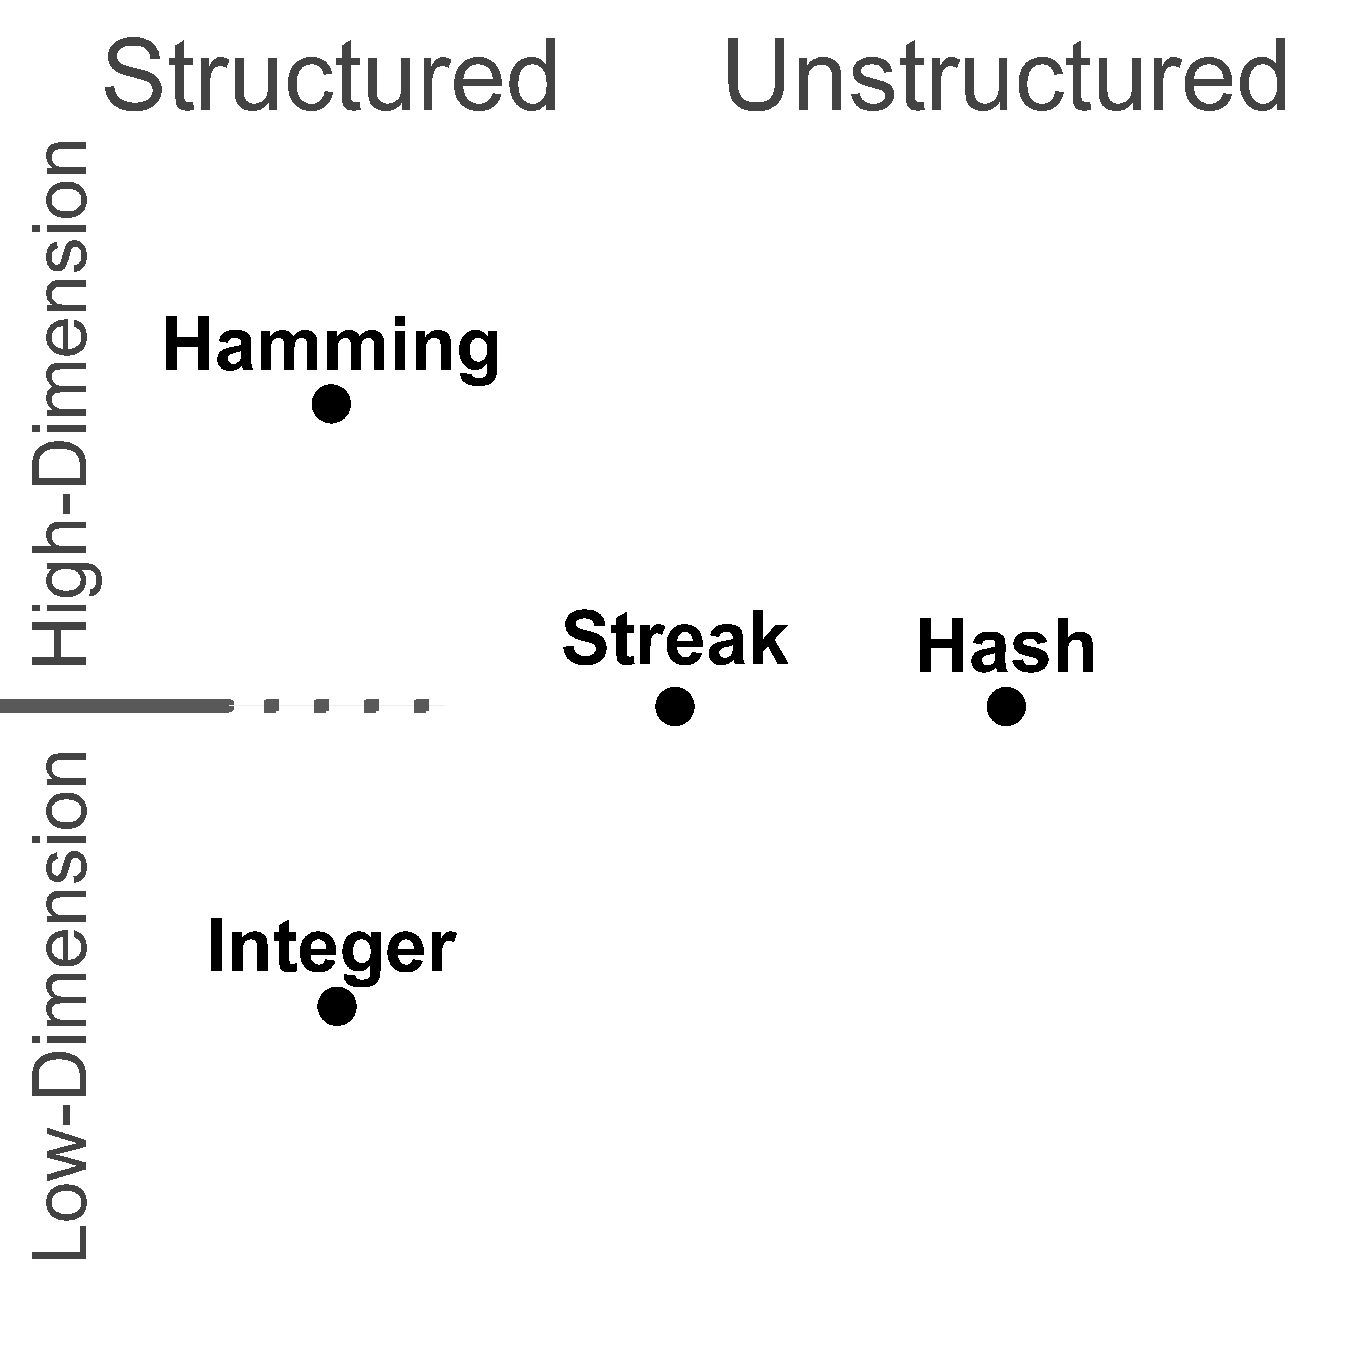
\includegraphics[width=\columnwidth]{img/conceptual-geometry}
\caption{
A conceptual schematic of the tag-matching metrics' geometric properties.
}
\label{fig:conceptual_geometry}

\end{center}
\end{figure}

% First, we performed  %TODO
% If two tags both closely match a third tag, will these two tags be constrained to closely match each other?
% Likewise, if a tag closely matches a second tag, will the tag be constrained to poorly match other tags the second tag poorly matches?
We used geometrical analyses to explore how tag-matching metrics constrain patterns of connectivity between tags, making some configurations unlikely or even impossible.
The bidirectional integer metric exhibited the tightest geometrical constraint in our analyses.
The unidirectional integer metric also exhibited tight geometrical constraint, but quirks of its non-commutative construction can allow that constraint to split across perfect- and worst-matching extremes.
Hamming and streak metrics exhibited looser geometric constraint, with the streak metric allowing for edge cases that very strongly break constraints.
Finally, the hash metric exhibited no geometrical constraint.

Next, we analyzed the effect of bitwise mutation on match distance score under the different metrics.
Under the hamming metric, all mutations have small effects on match distance score.
In contrast, under the integer metrics, rare mutations can have strong effects on match distance score.
The streak metric also exhibited strong-effect mutations, particularly with respect to coupling loosely-affiliated tags.
The hash metric exhibited the fattest tails of mutational magnitude, with strong-effect mutations occurring frequently.
Interestingly, the hash metric also exhibited sign-outcome frequencies that differed from the other metrics: mutations that decoupled tightly-matching tags and mutations that coupled loosely-matching tags were more frequent compared to other metrics.

The hamming metric exhibited the greatest robustness to mutation along mutational walks, followed by the streak metric.
The integer metrics, in particular the unidirectional integer metric, exhibited less robustness.
The streak metric, where all one-step mutations scramble match distance, exhibited the least robustness.

In evolutionary experiments, we found that network constraint (the number of tags a query or operand needs to simultaneously establish affinity with) differentially influenced performance of tag-matching metrics. 
In target-matching evolutionary experiments, netwowrk constraint corresponded to degree and regularity of the target graphs.
In the genetic programming experiments, this corresponded to the interconnectedness of module interaction networks that were selected for.

In target-matching evolutionary experiments, we found that the hash metric enabled rapid adaptive evolution toward targets with low network constraint.
This rapid evolution may be due to the hash metric's ability to rapidly generate variation.
In cases with high network constraint, however, the hash metric yielded poor-quality solutions.
The integer metrics also yielded poor-quality solutions for target graphs with network constraint.
In some more-constrained cases, the streak metric enabled more rapid adaptive evolution than the hamming metric.

In genetic programming evolutionary experiments, we found that the hamming and streak metrics yielded successful solutions the most frequently.
The hash metric had the next best performance, yielding more solutions than the integer metrics, which performed comparably.
On the directional signal task, which tends to require denser interaction networks, we found evidence that the streak metric enabled more rapid adaptive evolution than the hamming metric.

Relative to the other metrics, the streak metric tends to offer intermediate variational and geometric properties.
It exhibits some, but not strict, geometric constraint.
Many mutations are neutral or near-neutral (like the integer and hamming metrics) but a fat tail of extreme-effect mutations also occur (like the hash metric).
The streak metric exhibits robustness under mutational walks that falls between the hamming and integer metrics. 
However, it is unclear exactly why the streak metric enabled rapid adaptive evolution on the directional signal task.





\section{Conclusion}

we have characterized different tag schemes and demonstrated how they can have evolutionarily-observable consequences.

build stronger theory (evolvability and information-theory analysis)
\begin{enumerate}
\item  apply to understanding properties of biological e.g., proteins
\item  build a toolbox of tag matching schemes informed by theory
\item  modularity, duplication and differentiation, other things we didn't look at etc. etc.
\end{enumerate}

incorporate modular tag matching into artificial life models: open-source C++ tag-matching data structure implementation in Empirical with interchangeable metrics and selection algorithms

Holland notes tags as modular signal boundary systems \citep{holland2012signals}
This has been identified as a larger context of complex systems with parallels drawn to biology.
Insight into simple, abstract tag models might translate into a more nuanced appreciation of the principles underlying enzymatic protein-protein matchining biological systems.

On tag-matching constraint:
In a dynamically matched query-to-single-operand system, however, this can be relevant to the resulting connectivity under runtime silencing or upregulation of modules.
However, even in a static system, this can be relevant to resulting connectivity under deletion of an operand.



% \section{Software and Data Availability}

We implemented our experimental systems using the Empirical library for scientific software development in C++, available at \url{https://github.com/devosoft/Empirical} \citep{charles_ofria_2019_2575607}.
The code used to perform and analyze our experiments, our figures, and data from our experiments is available via the Open Science Framework at \url{https://osf.io/gw5mc/} \citep{foster2017open}.


\begin{acknowledgements}

Thanks to members of the DEVOLAB, in particular Nathan Rizik for help developing our tag-matching software infrastructure.
This research was supported by Michigan State University through the computational resources provided by the Institute for Cyber-Enabled Research.
This material is based upon work supported by the National Science Foundation Graduate Research Fellowship under Grant No. DGE-1424871.
Any opinions, findings, and conclusions or recommendations expressed in this material are those of the author(s) and do not necessarily reflect the views of the National Science Foundation.

\end{acknowledgements}

\footnotesize
\bibliographystyle{apalike}
\bibliography{bibl} % replace by the name of your .bib file

\clearpage
\newpage

\newgeometry{left=0.5in,right=0.5in,top=1in,bottom=1in}

\appendix

\setcounter{secnumdepth}{2}

\section{Supplementary Materials}

\begin{figure*}
\begin{center}

\includegraphics[width=\textwidth]{target_evolve/viz=max-fitness-bar+_data_hathash_hash=673d309ab90e91d1+_script_fullcat_hash=c9d2a8ac3d63fc8f+ext=}
\caption{
Maximum fitness among 50 replicate runs across a set of per-bit mutation rates.
Error bars represent 95\% confidence intervals.
}
\label{fig:evolve_mutsweep}

\end{center}
\end{figure*}


\begin{figure*}
\begin{center}

\includegraphics[width=\textwidth]{target_evolve_big/title=fitness_mutation_barplot+_data_hathash_hash=4db1200f9d71a980+_script_fullcat_hash=fe3ddc711c5abfad+ext=}
\caption{
Maximum fitness among replicate runs across a set of per-bit mutation rates.
Error bars represent 95\% confidence intervals.
}
\label{fig:evolve_big_mutsweep}

\end{center}
\end{figure*}



\footnotesize
\bibliographystyleinappendix{apalike}
\bibliographyinappendix{bibl} % replace by the name of your .bib file

\end{document}
